\chapter[Revisão Sistemática da Literatura]{Revisão Sistemática da Literatura}

A automação industrial tem testemunhado avanços exponenciais nas últimas décadas, impulsionada pela necessidade de aumentar a eficiência, a segurança e a produtividade em diversos setores. Nesse cenário, os \ac{VTA}, também chamados por \ac{RMT} ou mesmo \ac{UGV} emergem como ferramentas promissoras, particularmente em ambientes complexos e perigosos, como subestações elétricas. Essas instalações, essenciais para a distribuição de energia, apresentam desafios únicos para a operação humana e robótica, incluindo a necessidade de inspeções regulares de equipamentos, monitoramento de condições ambientais e segurança, e transporte de materiais em áreas de acesso restrito ou de alto risco. A capacidade de um \ac{UGV} navegar autonomamente nesses ambientes é, portanto, de suma importância, permitindo a execução dessas tarefas de forma mais eficiente, segura e com menor custo operacional. A navegação autônoma, neste contexto, refere-se à capacidade do robô de perceber seu entorno, localizar-se dentro dele, planejar e executar trajetórias seguras para atingir seus objetivos, tudo isso sem intervenção humana direta.
No entanto, a navegação autônoma em subestações elétricas e ambientes industriais similares é uma tarefa intrinsecamente complexa. Esses locais frequentemente combinam áreas internas e externas, formando ambientes parcialmente estruturados com corredores estreitos, espaços confinados e uma miríade de obstáculos. Equipamentos de alta tensão, estruturas metálicas, veículos de manutenção e a presença ocasional de pessoal criam um cenário dinâmico e desafiador. Obstáculos metálicos e superfícies reflexivas podem confundir sensores como \ac{LiDAR} e câmeras, enquanto a forte Interferência Eletromagnética ou \ac{EMI}, inerente a subestações, pode degradar severamente o desempenho de sensores eletrônicos e sistemas de comunicação sem fio, incluindo \ac{GPS}. Adicionalmente, as condições de iluminação podem variar drasticamente entre áreas internas e externas, dia e noite, e sob diferentes condições climáticas, exigindo sistemas de percepção robustos. A segurança é primordial, demandando que o sistema de navegação seja extremamente confiável para evitar colisões com equipamentos caros ou, mais criticamente, com pessoas.
Diante desses desafios, abordagens tradicionais de navegação autônoma, muitas vezes baseadas apenas em técnicas clássicas de Localização e Mapeamento Simultâneo ou \ac{SLAM} e planejamento de caminho determinístico, mostram-se insuficientes. Elas podem ter dificuldade em lidar com a dinâmica do ambiente, a incerteza dos sensores e a complexidade na tomada de decisões em tempo real. Surge, então, a necessidade de uma abordagem integrada que combine os avanços recentes em Aprendizado por Reforço, Visão Computacional e Fusão de Sensores. O Aprendizado por Reforço ou \ac{RL} oferece um paradigma poderoso para que o \ac{UGV} aprenda políticas de navegação complexas diretamente da interação com o ambiente (ou simulações dele), adaptando-se a situações imprevistas sem a necessidade de um modelo explícito pré-definido. A Visão Computacional, utilizando câmeras de baixo custo, fornece uma percepção rica e semanticamente densa do ambiente, permitindo ao robô não apenas detectar obstáculos, mas também compreender o contexto da cena. Por fim, a Fusão de Sensores é essencial para combinar as informações de múltiplas modalidades sensoriais como: \ac{LiDAR}, câmeras, radar, \ac{IMU}, explorando suas complementaridades para obter uma percepção mais robusta, precisa e confiável, mitigando as limitações individuais de cada sensor frente aos desafios do ambiente industrial.
O objetivo desta revisão de literatura é analisar criticamente o estado da arte, com foco no período entre 2015 e 2025, na integração sinérgica do Aprendizado por Reforço, Visão Computacional e Fusão de Sensores para o desenvolvimento de sistemas de navegação autônoma robustos e eficientes para \ac{UGV} operando em ambientes industriais desafiadores, com ênfase particular no contexto de subestações elétricas. Serão identificados e discutidos os principais algoritmos, metodologias, desafios persistentes e tendências emergentes nessas áreas e em sua intersecção. A estrutura desta revisão seguirá com uma seção dedicada ao contexto histórico (pré-2015), seguida por análises aprofundadas sobre Aprendizado por Reforço (Seção 2), Visão Computacional (Seção 3) e Fusão de Sensores (Seção 4) aplicadas à navegação de \ac{UGV}. A Seção 5 discutirá a integração dessas técnicas em sistemas completos, e a Seção 6 apresentará a conclusão e direções para pesquisas futuras.
Para contextualizar os avanços recentes, é importante revisitar brevemente o panorama da navegação autônoma antes de 2015, particularmente no período de 2006 a 2014. Essa era foi dominada por abordagens mais clássicas. O \ac{SLAM}, fundamental para robôs operando em ambientes desconhecidos, viu o desenvolvimento e refinamento de técnicas como \ac{SLAM} baseado em Filtro de Kalman Estendido (EKF-SLAM), Filtro de Partículas (FastSLAM), e métodos baseados em otimização gráfica (GraphSLAM). A navegação frequentemente dependia de mapas previamente construídos ou gerados por \ac{SLAM}, com algoritmos de planejamento de caminho como A*, D* e seus derivados sendo amplamente utilizados para encontrar rotas ótimas ou eficientes. Para a localização, Filtros de Kalman e Filtros de Partículas eram comumente empregados para fundir dados de odometria e sensores externos (como \textit{laser scanners}). No campo do aprendizado, o \textbf{\textit{Q-Learning}} tradicional era explorado, mas sua aplicação era limitada a espaços de estados e ações discretos e de baixa dimensionalidade. Embora essas técnicas tenham estabelecido as bases da navegação autônoma, suas limitações em lidar com ambientes altamente dinâmicos, incertezas complexas e a necessidade de comportamentos mais adaptativos motivaram fortemente a investigação e adoção das técnicas de \textit{Deep Learning} e Aprendizado por Reforço profundo que caracterizam a pesquisa mais recente, foco principal desta revisão.


\section{Aprendizado por Reforço (RL) e Aprendizado por Reforço Profundo (DRL)}
O Aprendizado por Reforço, ou \ac{RL} emergiu como uma abordagem promissora para enfrentar os desafios da navegação autônoma de \ac{UGV}, especialmente em ambientes complexos e dinâmicos como os encontrados em subestações elétricas. Diferentemente de métodos clássicos que dependem de modelos pré-definidos do ambiente ou regras heurísticas, o \ac{RL} permite que um agente \ac{UGV} aprenda uma política de controle ótima através da interação direta com seu ambiente (ou uma simulação dele), recebendo sinais de recompensa ou penalidade baseados em suas ações. Este paradigma de aprendizado por tentativa e erro é particularmente adequado para tarefas onde a dinâmica do ambiente é difícil de modelar explicitamente ou onde comportamentos adaptativos são necessários para lidar com incertezas e eventos imprevistos. A formulação padrão para problemas de \ac{RL} é o Processo de Decisão Markoviano, \ac{MDP}, que descreve a interação do agente com o ambiente em termos de estados (representações da situação atual do \ac{UGV} e do ambiente), ações (comandos de controle como velocidade e direção), recompensas (sinais que indicam o quão boa foi uma ação em um determinado estado) e uma política (a estratégia que o agente usa para selecionar ações com base nos estados, visando maximizar a recompensa acumulada a longo prazo).
A combinação do \ac{RL} com redes neurais profundas, conhecida como Aprendizado por Reforço Profundo, o \ac{DRL}, revolucionou o campo a partir de meados da década de 2010, permitindo que agentes aprendam políticas complexas diretamente a partir de entradas sensoriais de alta dimensionalidade, como imagens de câmeras ou dados de \ac{LiDAR}, superando as limitações do \ac{RL} tradicional em espaços de estados contínuos ou muito grandes. Diversos algoritmos \ac{DRL} se destacaram em aplicações de robótica e navegação. Entre os algoritmos baseados em valor, que aprendem uma função que estima o valor (recompensa futura esperada) de estar em um estado ou tomar uma ação em um estado, a \ac{DQN} foi um marco inicial. A \ac{DQN} utiliza uma rede neural profunda para aproximar a função Q (ação-valor) e emprega técnicas como \textit{experience replay} (armazenar e re-amostrar transições passadas) e \textit{target networks} (redes separadas para estabilizar o aprendizado) para lidar com dados correlacionados e instabilidades. No entanto, a \ac{DQN} original sofre de problemas como a superestimação dos valores Q. Extensões como \ac{DDQN}, que desacopla a seleção da ação da avaliação do valor, \textit{Dueling} \ac{DQN}, que separa a estimativa do valor do estado e da vantagem da ação, e \textit{Prioritized Experience Replay}, que amostra transições mais importantes com mais frequência, foram desenvolvidas para melhorar a estabilidade e o desempenho da \ac{DQN}. Esses métodos baseados em valor têm sido aplicados tanto em navegação baseada em mapas, onde o mapa é conhecido, quanto em navegação \textit{mapless}, onde o agente aprende a navegar apenas com base em suas percepções sensoriais imediatas.
Em contraste com os métodos baseados em valor, os algoritmos baseados em política aprendem diretamente uma política que mapeia estados para ações (ou uma distribuição de probabilidade sobre ações). Uma das abordagens mais populares e eficazes nesta categoria é a \ac{PPO}. A \ac{PPO} busca otimizar a política de forma mais estável, restringindo o tamanho das atualizações da política em cada etapa de treinamento através de uma função objetivo \textit{clipped} ou uma penalidade baseada na divergência de \ac{KL}. Isso evita mudanças drásticas na política que poderiam levar a um colapso no desempenho, tornando a \ac{PPO} particularmente adequada para problemas com espaços de ação contínuos, comuns no controle robótico, e relativamente mais fácil de implementar e ajustar em comparação com outros métodos de gradiente de política. Sua eficiência de dados e robustez a hiperparâmetros contribuíram para sua ampla adoção em tarefas de navegação.
Os métodos \textit{Actor-Critic} combinam elementos das abordagens baseadas em valor e em política. Eles utilizam dois componentes: um \textit{actor}, que representa a política e decide qual ação tomar, e um \textit{critic}, que avalia a ação tomada pelo \textit{actor} aprendendo uma função de valor (geralmente a função Q ou a função de valor do estado V). O \textit{critic} fornece um sinal de aprendizado para o \textit{actor}, guiando a atualização da política. O \ac{SAC} é um algoritmo \textit{Actor-Critic \textbf{off-policy}} que se destaca pela sua eficiência de amostra e estabilidade. Uma característica chave do \ac{SAC} é a incorporação de um termo de entropia na função objetivo, que encoraja a política a explorar mais amplamente, resultando em políticas mais robustas e evitando a convergência prematura para ótimos locais. Essa capacidade de exploração e a eficiência de dados tornam o SAC uma escolha atraente para tarefas complexas de controle robótico, incluindo a navegação autônoma.
Um dos maiores obstáculos na aplicação de \ac{DRL} em robótica no mundo real é o \textit{reality gap} – a discrepância entre o ambiente simulado onde o agente é frequentemente treinado (devido à segurança, custo e velocidade) e o ambiente real onde ele será implantado. Políticas treinadas puramente em simulação muitas vezes falham quando transferidas para o robô físico devido a diferenças na dinâmica do robô, nas características dos sensores (ruído, calibração), na aparência visual do ambiente e em outros fatores não modelados. As metodologias Sim-to-Real visam superar esse desafio. Uma técnica proeminente é a \textit{Domain Randomization}, que envolve a introdução de variabilidade significativa nos parâmetros da simulação durante o treinamento (parâmetros físicos como massa e atrito, texturas visuais, condições de iluminação, parâmetros dos sensores). A ideia é que, ao ser exposta a uma ampla gama de variações na simulação, a política aprendida se torne robusta o suficiente para operar no domínio real, que pode ser visto como apenas mais uma variação. Outras abordagens incluem a \textit{System Identification}, que tenta criar um modelo simulado mais preciso do robô e do ambiente real, e a Adaptação de Domínio (\textit{Domain Adaptation}), que utiliza técnicas para alinhar as distribuições de dados entre os domínios de simulação e real. Frequentemente, uma etapa final de \textit{fine-tuning} com uma pequena quantidade de dados coletados no robô real é utilizada para refinar a política aprendida na simulação. Diversos estudos têm demonstrado a eficácia das abordagens Sim-to-Real na transferência bem-sucedida de políticas de navegação para \ac{UGV}.
Além da eficácia, a segurança é uma preocupação primordial na navegação autônoma, especialmente em ambientes industriais onde falhas podem ter consequências graves. A engenharia de recompensas \textit{Reward Shaping} desempenha um papel crucial, onde a função de recompensa é cuidadosamente projetada para não apenas guiar o agente em direção ao objetivo, mas também para penalizar fortemente comportamentos indesejados, como colisões, proximidade excessiva de obstáculos ou zonas perigosas, e movimentos bruscos. No entanto, projetar recompensas perfeitas é desafiador. Por isso, o campo do \ac{RL} Seguro (\textit{Safe RL}) busca desenvolver algoritmos que possam garantir o cumprimento de restrições de segurança durante o processo de aprendizado e/ou execução. Abordagens incluem a formulação do problema como um \ac{MDP} com Restrições \ac{CMDP}, onde o objetivo é maximizar a recompensa enquanto se satisfaz restrições de custo (probabilidade de colisão abaixo de um limiar), o uso de funções de barreira Lyapunov ou Control Barrier Functions (CBFs) para garantir a permanência em um conjunto seguro de estados, ou a integração de controladores de segurança clássicos que podem intervir se a política de \ac{RL} propor uma ação insegura.
Finalmente, a aplicação de \ac{DRL} para navegação de \ac{UGV} em ambientes industriais específicos, como subestações, apresenta desafios particulares. O agente precisa aprender a navegar eficientemente em corredores estreitos, desviar de obstáculos metálicos que podem afetar sensores, lidar com a presença de pessoas ou outros veículos dinâmicos, e operar de forma robusta apesar da potencial interferência eletromagnética. A escalabilidade dos algoritmos \ac{DRL} para ambientes grandes e complexos, a necessidade de aprendizado contínuo para se adaptar a mudanças no layout ou nas condições operacionais, e a garantia de robustez e segurança a longo prazo permanecem áreas ativas de pesquisa e desenvolvimento.

\begin{figure}[H]
    \centering
    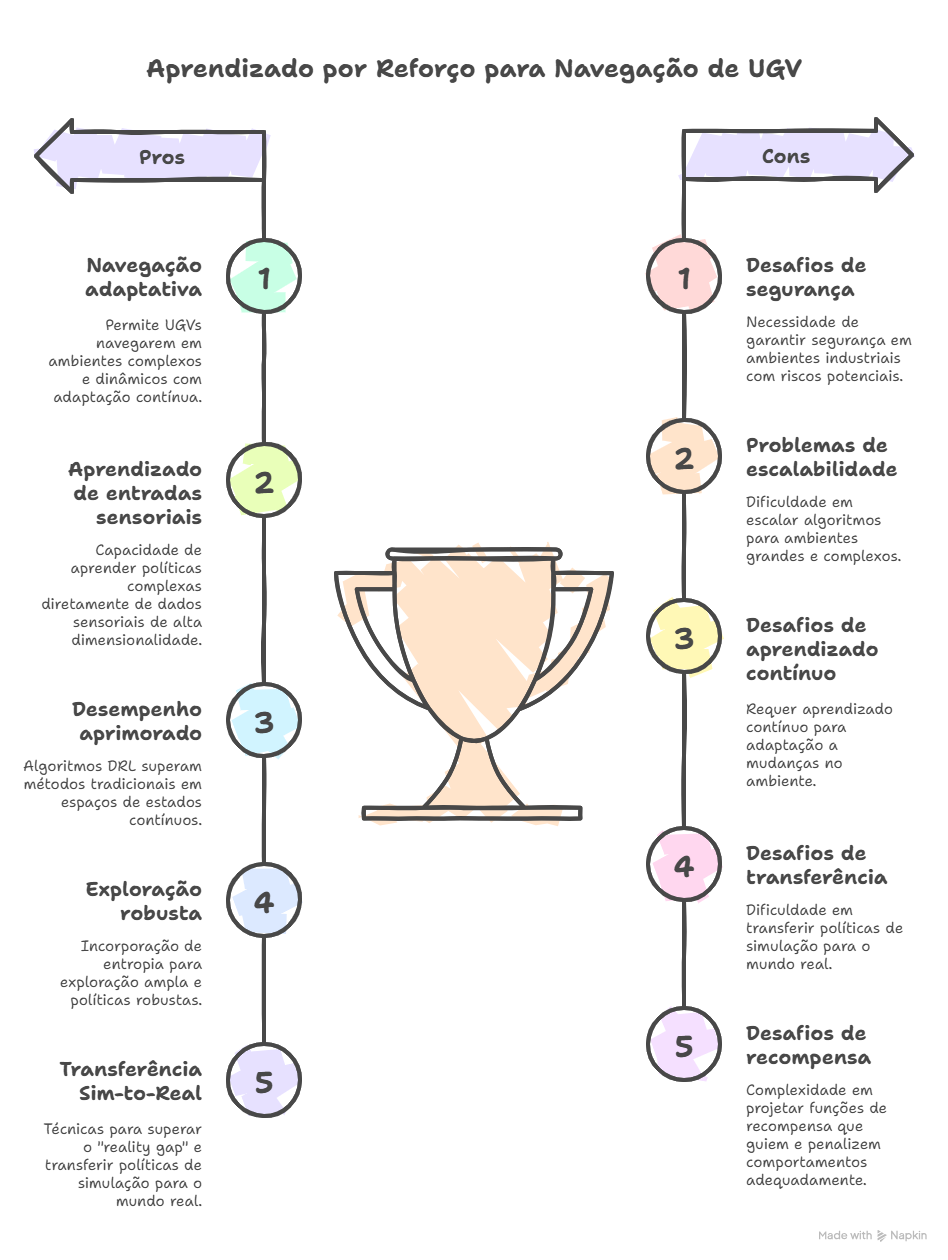
\includegraphics[width=0.8\textwidth]{figuras/aprendizado_reforco.png}
    \caption{Análise dos prós e contras do uso de Aprendizado por Reforço em sistemas de navegação autônoma para Robôs Móveis Terrestres. A figura destaca benefícios como a navegação adaptativa e a robustez na exploração, assim como desafios críticos relacionados à segurança, escalabilidade e transferência de políticas de simulação para o mundo real.}
    \legend{Fonte: O próprio autor.}
    \label{fig:aprendizado_reforco}    
\end{figure}

A Figura \ref{fig:aprendizado_reforco} acima apresenta uma análise dos principais aspectos positivos e negativos do uso de Aprendizado por Reforço na navegação autônoma de Robôs Móveis Terrestres. No lado esquerdo, destacam-se os benefícios, como a capacidade adaptativa dos \ac{UGV} em ambientes dinâmicos, o aprendizado direto de entradas sensoriais e a efetiva transferência de políticas de simulação para o mundo real. No lado direito, são evidenciados os desafios que ainda limitam a adoção prática, incluindo a necessidade de garantir segurança em ambientes industriais, a dificuldade de escalabilidade dos algoritmos para espaços maiores, e os entraves na definição e aplicação eficaz de funções de recompensa. A figura oferece uma visão resumida das vantagens e limitações que guiam o desenvolvimento de sistemas de navegação baseados em RL.

\section{Visão Computacional (CV) para Navegação Autônoma}
A Visão Computacional, ou \ac{CV}, desempenha um papel central na percepção de \ac{UGV} oferecendo uma fonte rica de informações sobre o ambiente a um custo relativamente baixo e de forma passiva. Utilizando câmeras (RGB, térmicas, de eventos, etc.), os sistemas de \ac{CV} podem extrair detalhes sobre a geometria da cena, identificar objetos, classificar terrenos e compreender o contexto geral, informações essenciais para a navegação autônoma segura e eficiente. Em ambientes industriais como subestações elétricas, onde a estrutura pode ser complexa e as condições operacionais desafiadoras, a capacidade da \ac{CV} de interpretar cenas visualmente é inestimável. No entanto, a percepção baseada em visão também enfrenta desafios significativos, incluindo sensibilidade a variações de iluminação, oclusões parciais ou totais de objetos, dificuldades na estimativa direta de distâncias 3D (especialmente com câmeras monoculares) e a necessidade de algoritmos robustos para interpretar dados visuais complexos e muitas vezes ambíguos.
Um dos desafios fundamentais para a navegação é a compreensão da geometria tridimensional do ambiente. A Estimativa de Profundidade Monocular, \ac{MDE}, visa inferir a distância de cada pixel na imagem em relação à câmera usando apenas uma única imagem como entrada. Este é um problema inerentemente mal posto, pois uma única imagem 2D pode corresponder a infinitas cenas 3D. No entanto, com o advento do \textit{Deep Learning}, progressos notáveis foram alcançados. Métodos supervisionados treinam redes neurais (frequentemente com arquiteturas \textit{encoder-decoder}, como U-Net) usando dados de treinamento que incluem mapas de profundidade precisos (geralmente obtidos com sensores \ac{LiDAR} ou estéreo). Por outro lado, métodos auto-supervisionados, que são particularmente atraentes devido à dificuldade de obter \textit{ground truth} de profundidade em larga escala, aprendem a estimar a profundidade explorando restrições geométricas a partir de sequências de vídeo (\textit{Structure from Motion}) ou pares de imagens estéreo (capturados ou sintéticos) como sinal de supervisão. Arquiteturas baseadas em \textit{Transformers} também têm sido exploradas para \ac{MDE}, aproveitando sua capacidade de modelar relações de longo alcance na imagem. Apesar dos avanços, a \ac{MDE} em ambientes industriais permanece desafiadora devido a texturas repetitivas ou ausentes, superfícies metálicas ou altamente reflexivas que violam as suposições de brilho constante, e mudanças abruptas de iluminação. Trabalhos recentes, como o \textit{Co-SemDepth} mencionado anteriormente (embora focado em \ac{UAV}, a arquitetura é relevante), exploram arquiteturas conjuntas que estimam profundidade e segmentação semântica simultaneamente, sugerindo que a compreensão semântica pode auxiliar na estimativa de profundidade e vice-versa, além de otimizar a eficiência computacional.
A Segmentação Semântica complementa a estimativa de profundidade ao fornecer uma compreensão do \textbf{o quê} está presente na cena, classificando cada pixel da imagem em categorias pré-definidas (chão navegável, obstáculo fixo, equipamento elétrico, parede, pessoa, veículo). Para a navegação autônoma, isso é crucial para identificar áreas seguras para locomoção, detectar e classificar obstáculos para planejamento de caminho reativo, e construir mapas semanticamente ricos do ambiente. Arquiteturas de \textit{Deep Learning}, como \ac{FCN}, U-Net e suas variantes (\textit{DeepLab} com convoluções \textit{atrous}), tornaram-se o padrão para segmentação semântica, alcançando alta precisão em diversos \textit{benchmarks}. Em ambientes industriais, a segmentação semântica enfrenta desafios como a aparência visual similar entre diferentes tipos de equipamentos ou estruturas, oclusões frequentes, a necessidade de definir e treinar modelos para classes de objetos específicas do domínio (que podem não estar presentes em \textit{datasets} genéricos) e a exigência de processamento em tempo real para garantir a segurança.
Recentemente, os Transformadores Visuais, ou \ac{ViT}, inspirados no sucesso dos \textit{Transformers} em Processamento de Linguagem Natural, ou \ac{NLP}, emergiram como uma alternativa poderosa às Redes Neurais Convolucionais, conhecidas como \ac{CNN} para tarefas de visão. A arquitetura \ac{ViT} básica divide a imagem em \textit{patches}, os projeta linearmente e os processa através de blocos \textit{Transformer} padrão, que utilizam mecanismos de auto-atenção para capturar dependências globais entre os \textit{patches}. Essa capacidade de modelar relações de longo alcance é uma vantagem potencial sobre as \ac{CNN}, que têm um campo receptivo inerentemente local. Variações como o \textit{Swin Transformer} introduziram janelas de atenção deslocadas para melhorar a eficiência e capturar informações em diferentes escalas. Para aplicações industriais onde a eficiência de implantação é crítica, arquiteturas híbridas ou otimizadas como o \textit{Next-ViT} foram propostas. O \textit{Next-ViT} combina blocos convolucionais eficientes, ou \ac{NCB} para capturar informações locais com blocos \textit{Transformer} ou \ac{NTB} para modelar dependências globais, utilizando uma estratégia híbrida, ou \ac{NHS} para empilhá-los de forma otimizada para o \textit{trade-off} latência/precisão em plataformas de hardware comuns como \textit{TensorRT} e \textit{CoreML}. A aplicabilidade dos \ac{ViT} na navegação de \ac{UGV} reside em seu potencial para uma compreensão mais holística da cena, o que pode beneficiar tarefas como detecção de obstáculos distantes, análise de contexto e planejamento de longo prazo, embora seu custo computacional e a necessidade de grandes \textit{datasets} para treinamento ainda sejam considerações importantes.
Em suma, a Visão Computacional oferece capacidades indispensáveis para a percepção de \ac{UGV} em subestações elétricas, mas enfrenta desafios específicos relacionados ao ambiente. A oclusão por equipamentos densamente instalados, os reflexos em superfícies metálicas que podem criar artefatos visuais ou confundir algoritmos de \ac{MDE}, as condições de iluminação variáveis e por vezes precárias, e a presença de poeira, vapor ou outros particulados que degradam a qualidade da imagem, exigem algoritmos de \ac{CV} robustos e adaptativos. A combinação de diferentes técnicas de \ac{CV} (\ac{MDE}, segmentação, detecção de objetos) e a integração com outros sensores através da fusão são estratégias chave para superar essas limitações e alcançar a percepção confiável necessária para a navegação autônoma segura em ambientes industriais complexos.

\begin{figure}[H]
    \centering
    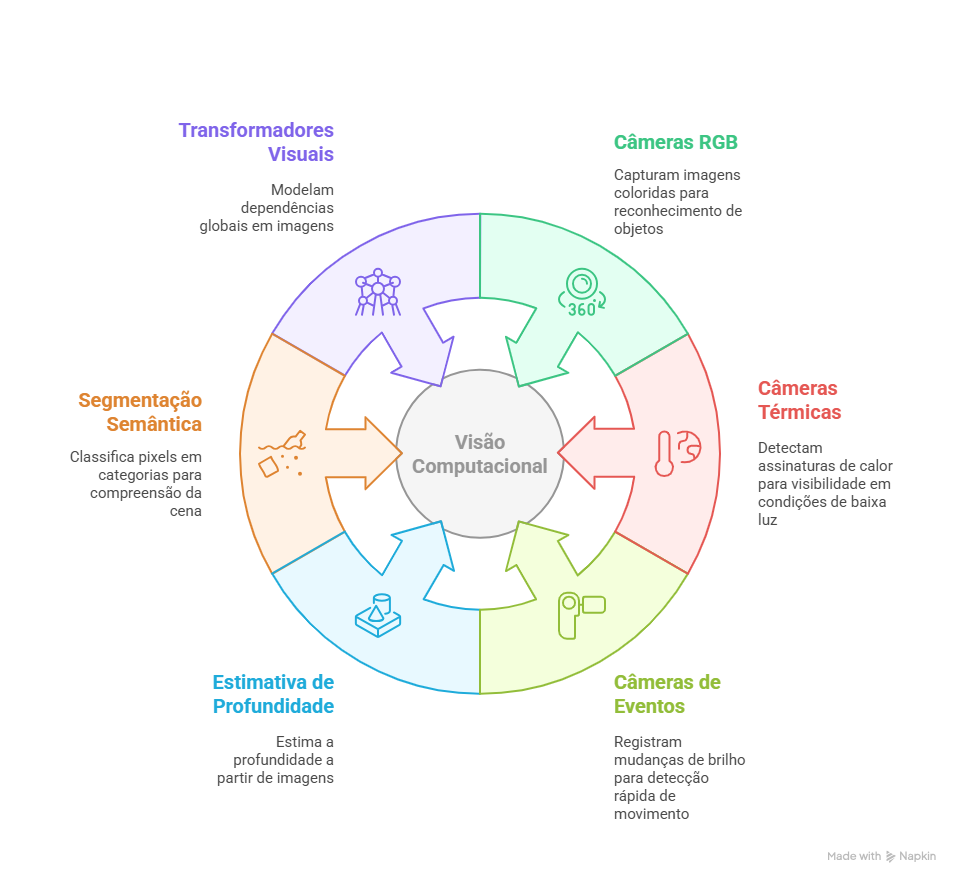
\includegraphics[width=0.90\textwidth]{figuras/visao_computacional.png}
    \caption{Componentes visuais e sensores utilizados na percepção de Robôs Móveis Terrestres. A figura ilustra as principais tecnologias aplicadas à Visão Computacional, como câmeras RGB, térmicas e de eventos, além de métodos computacionais como estimativa de profundidade, segmentação semântica e transformadores visuais, que juntos contribuem para uma compreensão robusta do ambiente.}
    \legend{Fonte: O próprio autor.}
    \label{fig:visao_computacional}
\end{figure}

A Figura \ref{fig:visao_computacional} acima apresenta os principais elementos que compõem a percepção visual de Robôs Móveis Terrestres em ambientes complexos. São destacados diferentes tipos de câmeras (RGB, térmicas e de eventos), cada uma com características específicas para captar informações visuais sob variadas condições ambientais. Adicionalmente, a figura mostra técnicas de processamento, como Estimativa de Profundidade, Segmentação Semântica e Transformadores Visuais, fundamentais para que o robô interprete seu entorno de forma precisa e confiável. Essa combinação de sensores e algoritmos viabiliza uma navegação autônoma mais segura, especialmente em ambientes industriais como subestações elétricas.

\section{Fusão de Sensores}
A confiança exclusiva em um único tipo de sensor para a percepção ambiental em \ac{UGV} é frequentemente inadequada, especialmente nos ambientes industriais complexos e adversos como subestações elétricas. Cada modalidade sensorial possui suas próprias forças e fraquezas inerentes. Por exemplo, enquanto o \ac{LiDAR} fornece medições geométricas 3D precisas, pode ser afetado por condições atmosféricas como chuva ou neblina e ter dificuldade com superfícies transparentes ou altamente reflexivas, além de não fornecer informações semânticas ricas. As câmeras RGB oferecem dados texturais e semânticos densos, mas são sensíveis a variações de iluminação e não medem diretamente a profundidade. O radar é robusto a condições climáticas adversas e pode medir velocidades, mas geralmente possui baixa resolução angular. A \ac{IMU} fornece informações sobre o movimento próprio do robô, mas sofre de acumulação de erro (\textit{drift}) ao longo do tempo. A Fusão de Sensores surge como uma estratégia indispensável para superar as limitações individuais, explorando a complementaridade das diferentes modalidades sensoriais para alcançar uma percepção do ambiente mais robusta, precisa, completa e confiável. Ao combinar informações de múltiplos sensores, o sistema pode aumentar a cobertura espacial e temporal, melhorar a precisão das estimativas, aumentar a robustez a falhas de sensores individuais e obter uma compreensão mais rica e holística do ambiente.
Para \ac{UGV} operando em ambientes industriais, um conjunto típico de sensores inclui \ac{LiDAR}, câmeras (RGB, térmicas, de eventos), radar e \ac{IMU}. O \ac{LiDAR}, geralmente utilizando lasers pulsados, mede distâncias com alta precisão, gerando nuvens de pontos 3D detalhadas do ambiente, sendo fundamental para mapeamento e detecção de obstáculos geométricos. Câmeras RGB são onipresentes devido ao seu baixo custo e riqueza de informações visuais e semânticas. Câmeras térmicas podem ser valiosas em subestações para detectar superaquecimento em equipamentos ou a presença de pessoas/animais em condições de baixa visibilidade. Câmeras baseadas em eventos, que detectam mudanças de intensidade luminosa em cada pixel de forma assíncrona, oferecem alta faixa dinâmica e baixa latência, sendo promissoras para ambientes com iluminação desafiadora ou movimentos rápidos. O radar, utilizando ondas de rádio, é particularmente valioso por sua capacidade de operar em condições climáticas adversas (chuva, neblina, poeira) e medir diretamente a velocidade radial dos objetos, embora com menor resolução espacial que o \ac{LiDAR} ou câmeras. A \ac{IMU}, composta por acelerômetros e giroscópios, mede a aceleração linear e a velocidade angular do robô, sendo crucial para a estimativa de estado (pose, velocidade) em curtos intervalos de tempo e para a fusão com outros sensores para localização (odometria visual-inercial ou LiDAR-inercial). Sensores adicionais como ultrassom (para detecção de obstáculos de curto alcance) e GPS (para localização global em áreas externas, se o sinal não for bloqueado ou afetado por \ac{EMI}) também podem ser incorporados.
A fusão das informações provenientes desses diversos sensores pode ocorrer em diferentes níveis de abstração. A Fusão de Dados Brutos (\textit{Low-Level Fusion}) tenta combinar os dados brutos dos sensores antes de qualquer processamento significativo. Embora potencialmente possa preservar o máximo de informação, é computacionalmente intensiva e sensível a ruídos e erros de calibração. A Fusão de Características (\textit{Mid-Level Fusion}) envolve a extração de características relevantes de cada sensor (bordas, cantos de imagens; planos, segmentos de nuvens de pontos LiDAR) e a fusão dessas características em um espaço comum. Esta abordagem oferece um bom equilíbrio entre preservação de informação e complexidade computacional. A Fusão de Decisões (\textit{High-Level Fusion}), também conhecida como fusão de objetos ou de trilhas, processa os dados de cada sensor independentemente para gerar detecções de objetos ou estimativas de estado, que são então combinadas em um estágio final para produzir uma decisão ou estimativa global. Esta abordagem é modular e robusta a falhas de sensores individuais, mas pode perder informações correlacionadas presentes nos dados brutos ou características.
Diversas técnicas matemáticas e algorítmicas são empregadas para realizar a fusão. Abordagens clássicas baseadas em filtros probabilísticos são amplamente utilizadas, especialmente para estimativa de estado (localização e rastreamento). O Filtro de \textit{Kalman}, ou \ac{KF} e suas extensões para sistemas não lineares, como o Filtro de \textit{Kalman} Estendido, o \ac{EKF} e o Filtro de \ac{UKF}, fornecem um \textit{framework} ótimo (sob certas suposições) para fundir medições ruidosas de múltiplos sensores e estimar o estado de um sistema dinâmico. Filtros de Partículas, ou \ac{PF} oferecem uma alternativa para sistemas com não-linearidades fortes ou distribuições de probabilidade não-Gaussianas. Mais recentemente, técnicas baseadas em \textit{Deep Learning} têm ganhado destaque para fusão de sensores, particularmente para tarefas como detecção e segmentação de objetos multimodais. Redes neurais podem ser projetadas para aceitar entradas de diferentes sensores e aprender a combinar suas características em representações intermediárias (fusão por concatenação, soma ou mecanismos de atenção) ou fundir as saídas de redes específicas de cada modalidade. Essas abordagens têm o potencial de aprender correlações complexas entre os dados dos sensores de forma automática, mas requerem grandes quantidades de dados de treinamento multimodais anotados.
Um pré-requisito fundamental para qualquer sistema de fusão de sensores é a calibração precisa. A Calibração Intrínseca refere-se à determinação dos parâmetros internos de cada sensor (distância focal e centro óptico de uma câmera, bias e ruído de uma \ac{IMU}). A Calibração Extrínseca envolve a determinação precisa da transformação espacial (rotação e translação) entre os sistemas de coordenadas dos diferentes sensores (e.g., a pose relativa entre um\ac{LiDAR} e uma câmera, ou entre uma câmera e uma \ac{IMU}). Erros na calibração extrínseca podem degradar severamente o desempenho da fusão, levando a desalinhamentos entre os dados dos sensores e, consequentemente, a uma percepção incorreta do ambiente. A calibração pode ser realizada \textit{offline}, mas a calibração online ou auto-calibração, que ajusta continuamente os parâmetros durante a operação, é desejável para lidar com variações devido a temperatura ou vibrações.
Além da calibração, a operação em tempo real é um requisito crítico para a navegação autônoma. Os algoritmos de fusão e percepção devem ser capazes de processar os fluxos de dados dos sensores e gerar informações relevantes para o planejamento e controle em uma taxa compatível com a dinâmica do \ac{UGV} e do ambiente. Isso impõe restrições significativas sobre a complexidade computacional dos algoritmos, especialmente considerando as limitações de poder de processamento e consumo de energia das plataformas embarcadas típicas de \ac{UGV}. A otimização de algoritmos e o uso de hardware especializado (como as \ac{FPGA} ou como as GPUs embarcadas) são frequentemente necessários.
Finalmente, a fusão de sensores em ambientes industriais como subestações elétricas apresenta desafios adicionais. A sincronização temporal precisa dos dados provenientes de sensores com diferentes taxas de amostragem é crucial. O sistema deve ser robusto a falhas parciais ou totais de sensores individuais, utilizando a redundância fornecida pela multiplicidade de sensores. O impacto da Interferência Eletromagnética \ac{EMI} na qualidade dos dados de certos sensores (\ac{IMU}, \ac{GPS}, comunicação sem fio) precisa ser considerado e mitigado, possivelmente através de blindagem, filtragem ou algoritmos de fusão robustos a \textit{outliers}. A complexidade inerente à integração, manutenção e diagnóstico de um sistema com múltiplos sensores também representa um desafio de engenharia significativo.

\begin{figure}[H]
    \centering
    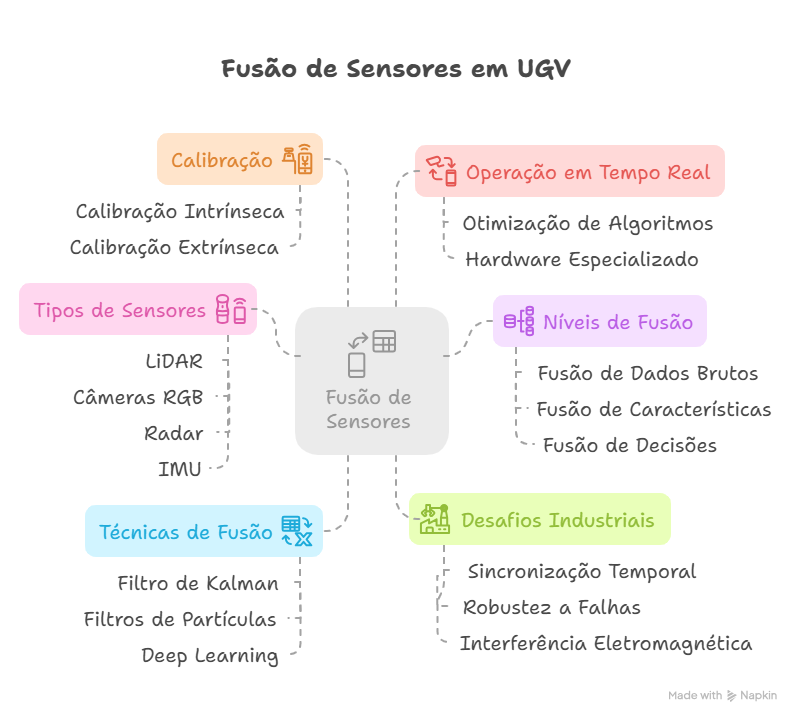
\includegraphics[width=0.90\textwidth]{figuras/fusao_sensores.png}
    \caption{Aspectos fundamentais da Fusão de Sensores em UGV. A figura apresenta os principais tipos de sensores, técnicas de fusão, níveis de integração, e desafios enfrentados, como calibração precisa, operação em tempo real e robustez frente a interferências industriais.}
    \legend{Fonte: O próprio autor.}
    \label{fig:fusao_sensores}
\end{figure}

A Figura \ref{fig:fusao_sensores} resume os principais componentes envolvidos na fusão de sensores para Robôs Móveis Terrestres. São apresentados os diferentes tipos de sensores (LiDAR, câmeras RGB, radar, IMU) utilizados para fornecer informações complementares sobre o ambiente. A figura também destaca os níveis de fusão (dados brutos, características e decisões) e as técnicas mais comuns, como filtros de Kalman, filtros de partículas e métodos baseados em Deep Learning. Além disso, são abordados os principais desafios industriais, como a necessidade de sincronização temporal, robustez a falhas e interferência eletromagnética, e a exigência de uma operação em tempo real eficiente com o suporte de algoritmos otimizados e hardware especializado.

\section{Conclusão e Direções Futuras}
Esta revisão de literatura analisou o estado da arte na integração de Aprendizado por Reforço, Visão Computacional e Fusão de Sensores para a navegação autônoma de Robôs Móveis Terrestres em ambientes industriais desafiadores, com foco particular em subestações elétricas, cobrindo principalmente o período de 2015 a 2025. A crescente demanda por automação nessas instalações, aliada aos riscos e complexidades inerentes, impulsiona a necessidade de sistemas de navegação robustos e inteligentes. A análise revelou que, embora abordagens clássicas tenham estabelecido fundamentos importantes, a combinação das três áreas tecnológicas em foco oferece um potencial significativo para superar as limitações existentes.
O Aprendizado por Reforço Profundo demonstrou capacidade para aprender políticas de navegação complexas em ambientes com dinâmicas difíceis de modelar, com algoritmos como DQN, PPO e SAC mostrando-se promissores. As metodologias \textit{Sim-to-Real} são cruciais para viabilizar o treinamento em simulação e a transferência para o mundo real, enquanto a engenharia de recompensas e as técnicas de \ac{RL} Seguro são essenciais para garantir a operação confiável e segura em ambientes críticos. A Visão Computacional, por sua vez, fornece percepção rica do ambiente, com avanços notáveis em Estimativa de Profundidade Monocular, Segmentação Semântica e o surgimento dos Transformadores Visuais oferecendo novas possibilidades para a compreensão de cena. No entanto, desafios como variações de iluminação, oclusões e superfícies reflexivas persistem em ambientes industriais. A Fusão de Sensores é indispensável para mitigar as fraquezas de sensores individuais, combinando dados de \ac{LiDAR}, câmeras, radar e \ac{IMU} através de técnicas baseadas em filtros ou aprendizado profundo para obter uma percepção robusta. A calibração precisa e a sincronização temporal são pré-requisitos fundamentais, e a robustez a falhas e interferências (como \ac{EMI}) é uma consideração crítica.
A integração dessas três áreas é onde reside o maior potencial, mas também os maiores desafios. Utilizar a percepção avançada da \ac{CV} e da fusão de sensores para criar representações de estado informativas para o \ac{RL}, ou usar o \ac{RL} para aprender políticas de controle adaptativas ou até mesmo estratégias de fusão, são direções promissoras. A literatura recente começa a explorar essas sinergias, mas sistemas completos que integram robustamente todas as componentes em \ac{UGV} operando em subestações reais ainda são relativamente escassos.
Apesar dos progressos significativos, diversas lacunas e desafios permanecem. A robustez a longo prazo e a capacidade de adaptação contínua a mudanças no ambiente (novos equipamentos, layouts modificados) ainda são limitadas. A maioria dos trabalhos de \ac{RL} foca em tarefas específicas ou ambientes simulados, e a validação em cenários industriais reais e complexos, como subestações operacionais, ainda é um gargalo. A falta de \textit{datasets} e \textit{benchmarks} padronizados especificamente para \ac{UGV} em subestações elétricas dificulta a comparação objetiva de diferentes abordagens. A segurança, embora abordada pelo \ac{RL} Seguro, ainda requer métodos mais formalmente verificáveis e garantias mais fortes para implantação em ambientes de alto risco. A explicabilidade e interpretabilidade ou \ac{XAI} dos modelos de DRL e \ac{CV} profundos aplicados à navegação são áreas emergentes, mas cruciais para a certificação e aceitação desses sistemas.
Com base nessas lacunas, diversas direções futuras de pesquisa podem ser delineadas. Primeiramente, o desenvolvimento de técnicas Sim-to-Real mais eficazes e eficientes em termos de dados, possivelmente combinando \textit{domain randomization} com adaptação de domínio online e aprendizado contínuo a partir de interações reais limitadas, é fundamental. Em segundo lugar, a pesquisa em \ac{RL} Seguro precisa avançar para fornecer garantias mais fortes e métodos escaláveis para problemas de navegação complexos com múltiplas restrições. Terceiro, a exploração de arquiteturas de fusão multimodal mais sofisticadas, que possam aprender dinamicamente a ponderar a contribuição de cada sensor com base no contexto e na confiabilidade estimada, é promissora. Isso inclui a integração mais profunda de sensores proprioceptivos (como odometria de roda e \ac{IMU}) e exteroceptivos, e potencialmente informações de comunicação \ac{V2X} se disponíveis. Quarto, a investigação em \ac{XAI} aplicada a sistemas de navegação baseados em \ac{DRL} e \ac{CV} é necessária para entender como e porquê os sistemas tomam certas decisões, aumentando a confiança e facilitando a depuração. Quinto, a otimização contínua de algoritmos para hardware embarcado com restrições de energia e computação é essencial para a viabilidade prática. Finalmente, estender a navegação autônoma de um único \ac{UGV} para a coordenação e navegação colaborativa de múltiplos \ac{UGV} em ambientes industriais abre novas possibilidades para tarefas complexas, mas também introduz desafios adicionais em comunicação, planejamento conjunto e gerenciamento de interferências.
Em conclusão, a convergência do Aprendizado por Reforço, Visão Computacional e Fusão de Sensores está pavimentando o caminho para a próxima geração de sistemas de navegação autônoma para \ac{UGV}. Embora desafios significativos permaneçam, especialmente na transição para ambientes industriais reais como subestações elétricas, a pesquisa contínua nessas áreas e em sua integração sinérgica promete viabilizar robôs mais inteligentes, robustos e seguros, capazes de realizar tarefas complexas e perigosas, transformando as operações industriais no futuro próximo.

\begin{table}[H]
    \centering
    \caption{Síntese da Revisão da Literatura sobre Navegação Autônoma de UGVs.}
    \label{tab:sintese_literatura}
    \begin{tabularx}{\textwidth}{|l|X|X|X|}
        \hline
        \textbf{Área} & \textbf{Aspectos Abordados} & \textbf{Desafios Identificados} & \textbf{Principais Referências} \\
        \hline
        Aprendizado por Reforço & 
        - DQN, DDQN, PPO, SAC \newline 
        - Políticas adaptativas \newline 
        - Safe RL e CMDPs \newline 
        - Sim-to-Real, Domain Randomization &
        - Garantia de segurança em ambientes industriais \newline 
        - Escalabilidade para ambientes grandes \newline 
        - Transferência para o mundo real &
        Sutton \& Barto (2018); Zhang et al. (2023); Huang et al. (2021, 2023); AlMahamid \& Grolinger (2024) \\
        \hline
        Visão Computacional &
        - Estimativa de profundidade monocular \newline 
        - Segmentação semântica \newline 
        - Vision Transformers (ViT) \newline 
        - Câmeras RGB, térmicas e de eventos &
        - Variação de iluminação \newline 
        - Oclusões e superfícies reflexivas \newline 
        - Exigência de tempo real &
        Tang et al. (2020); Zieliński \& Markowska-Kaczmar (2021); Florea et al. (2022); Li et al. (2025) \\
        \hline
        Fusão de Sensores &
        - Fusão em níveis: dados brutos, características, decisões \newline 
        - Filtros de Kalman, Filtros de Partículas, Deep Learning \newline 
        - Calibração e sincronização &
        - Robustez frente à EMI \newline 
        - Otimização computacional \newline 
        - Falhas parciais de sensores &
        Fayyad et al. (2020); Yeong et al. (2021); Xiang et al. (2023); Jahromi et al. (2019) \\
        \hline
        Ambiente Industrial (Subestações) &
        - Corredores estreitos e obstáculos metálicos \newline 
        - Interferência eletromagnética severa \newline 
        - Ambientes internos e externos mistos &
        - Necessidade de validação prática \newline 
        - Falta de datasets específicos \newline 
        - Adaptação contínua a mudanças no layout &
        Revisão geral baseada em gaps identificados \\
        \hline
    \end{tabularx}
    \legend{Fonte: O próprio autor.}
\end{table}

A Tabela \ref{tab:sintese_literatura} apresenta uma síntese da revisão da literatura realizada, organizada por áreas temáticas centrais para o desenvolvimento de sistemas de navegação autônoma de UGVs em ambientes industriais. Em cada área — Aprendizado por Reforço, Visão Computacional, Fusão de Sensores e especificidades do ambiente de subestações elétricas — são destacados os principais aspectos abordados pelos autores, os desafios recorrentes encontrados na literatura e as referências mais relevantes que fundamentam a discussão. Esta tabela oferece uma visão integrada e resumida do estado da arte, auxiliando o leitor na compreensão das conexões entre as tecnologias analisadas e as lacunas que justificam a proposta desta pesquisa.

\begin{table}[H]
    \centering
    \caption{Lacunas e Oportunidades de Pesquisa na Navegação Autônoma de UGV apoiadas por Aprendizagem por Reforço, Visão Computacional e Fusão de Sensores.}
    \label{tab:lacunas_oportunidades}
    \begin{tabularx}{\textwidth}{|>{\hsize=0.33\hsize}X|>{\hsize=0.67\hsize}X|}
        \hline
        \textbf{Lacuna Identificada} & \textbf{Descrição e Oportunidades de Pesquisa} \\
        \hline
        Robustez em longo prazo e adaptabilidade contínua & Sistemas atuais são limitados frente a mudanças frequentes em subestações. É necessário desenvolver algoritmos que permitam adaptação contínua e operação confiável a longo prazo. \\
        \hline
        Validação prática em subestações elétricas reais & Poucos estudos testam em ambientes reais. Oportunidade para validação prática com foco em desafios específicos como EMI e obstáculos metálicos. \\
        \hline
        Falta de datasets e benchmarks padronizados & Inexistência de bases de dados específicas para UGVs em subestações. Potencial para criar datasets públicos que permitam comparações entre soluções. \\
        \hline
        Garantias formais e segurança robusta & Faltam métodos com garantias matemáticas de segurança. Necessidade de RL seguro mais rigoroso, com validação formal. \\
        \hline
        Explicabilidade e interpretabilidade (XAI) & Limitações na compreensão de decisões de DRL e CV. Pesquisas em XAI podem facilitar aceitação industrial e certificação. \\
        \hline
        Técnicas eficazes de Sim-to-Real & Transferência do simulado ao real ainda ineficiente. Oportunidade para explorar randomização de domínio e aprendizado incremental. \\
        \hline
        Fusão adaptativa e dinâmica de sensores & Predomínio de esquemas estáticos. Desenvolver fusão que ajuste dinamicamente a influência dos sensores conforme condições ambientais. \\
        \hline
        Otimização computacional para hardware embarcado & Alta demanda computacional de algoritmos atuais. Desafio em otimizar para operação eficiente em plataformas embarcadas. \\
        \hline
        Coordenação colaborativa entre múltiplos UGVs & Pouca pesquisa em navegação conjunta de vários UGVs em subestações. Oportunidade para explorar estratégias colaborativas e comunicação entre robôs. \\
        \hline
    \end{tabularx}
    \legend{Fonte: O próprio autor.}
\end{table}

A Tabela \ref{tab:lacunas_oportunidades} apresenta as principais lacunas e oportunidades de pesquisa identificadas na revisão da literatura sobre navegação autônoma de UGVs em ambientes industriais, com ênfase em subestações elétricas. Cada lacuna destacada representa uma limitação dos sistemas atuais e aponta direções promissoras para o avanço científico e tecnológico na área. Essas oportunidades abrangem desde desafios técnicos, como a robustez a longo prazo e a fusão adaptativa de sensores, até questões práticas, como a validação em ambientes reais e a criação de benchmarks padronizados. Essa síntese orienta o escopo da pesquisa e justifica as contribuições potenciais do trabalho em desenvolvimento.